\documentclass[12pt]{article}
\usepackage[utf8]{inputenc}
\usepackage{geometry}
\geometry{a4paper, margin=1in}
\usepackage{graphicx}
\usepackage{hyperref}
\usepackage[english]{babel}
\usepackage{pgfplots}
\usepackage{array}
\pgfplotsset{compat=1.18} 

\title{Extended Memorandum for Project 0002}
\author{Project Manager: Juan Pérez}
\date{September 24, 2024}

\begin{document}

\maketitle

\tableofcontents
\newpage

\section{Executive Summary}
This memorandum provides a comprehensive overview of the ABC project. It covers the context, progress, risks, and challenges. Additionally, a detailed analysis of the schedule and budget is presented. A comparison of the initial plan with the current state will also be provided, highlighting deviations and risk mitigation strategies.

\section{Context}
The ABC project was initiated to address inefficiencies in the existing system. The project aims to improve system performance by 30%, reduce downtime, and enhance user experience. The project officially began on July 1, 2024, with an expected completion date in December 2024.

The project involves several teams, including software development, quality assurance, and project management. The main objectives are:
\begin{itemize}
    \item Improve system performance by 30%.
    \item Enhance user experience with a redesigned interface.
    \item Reduce system downtime by 50%.
    \item Ensure data synchronization across platforms.
\end{itemize}

\section{Progress to Date}
The project is currently in its second phase, with 60\% of the development work completed. Below is a breakdown of the work done to date:

\begin{itemize}
    \item \textbf{Phase 1: Requirements Gathering} (Completed on August 15, 2024)
    \item \textbf{Phase 2: Development} (60\% completed, expected completion by October 15, 2024)
    \item \textbf{Phase 3: Testing and Implementation} (Scheduled for November - December 2024)
\end{itemize}

\section{Project Timeline and Milestones}
The following table provides a detailed timeline of project milestones and completion percentages:

\begin{center}
\begin{table}[h]
\small
% \fontsize{10pt}{10pt}\selectfont
\begin{tabular}{|m{4cm}|m{4cm}|m{4cm}|m{2cm}|}
\hline
\textbf{Milestone} & \textbf{Planned Date} & \textbf{Actual Date} & \textbf{Status} \\
\hline
Requirements Gathering & August 15, 2024 & August 15, 2024 & 100\% \\
\hline
User Authentication & September 1, 2024 & September 5, 2024 & 100\% \\
\hline
API Integration & October 1, 2024 & In progress & 50\% \\
\hline
Testing Phase & November 15, 2024 & To be determined & Not Started \\
\hline
Final Implementation & December 15, 2024 & To be determined & Not Started \\
\hline
\end{tabular}
\end{table}
\end{center}

\section{Budget Analysis}
The project budget has remained within limits, although delays in API integration could impact costs. Below is a breakdown of the allocated versus actual budget for each phase.

\begin{itemize}
    \item \textbf{Total Budget:} \$500,000
    \item \textbf{Amount Spent:} \$300,000 (As of September 24, 2024)
\end{itemize}

\subsection*{Detailed Budget Breakdown}
\begin{itemize}
    \item Requirements Gathering: \$100,000 (Spent: \$95,000)
    \item Development: \$250,000 (Spent: \$150,000)
    \item Testing: \$100,000 (Allocated)
    \item Implementation: \$50,000 (Allocated)
\end{itemize}

\section{Current Status}
The development phase is ongoing, focused on API integration. Below is a Gantt chart providing a visual representation of the project schedule.

\begin{center}
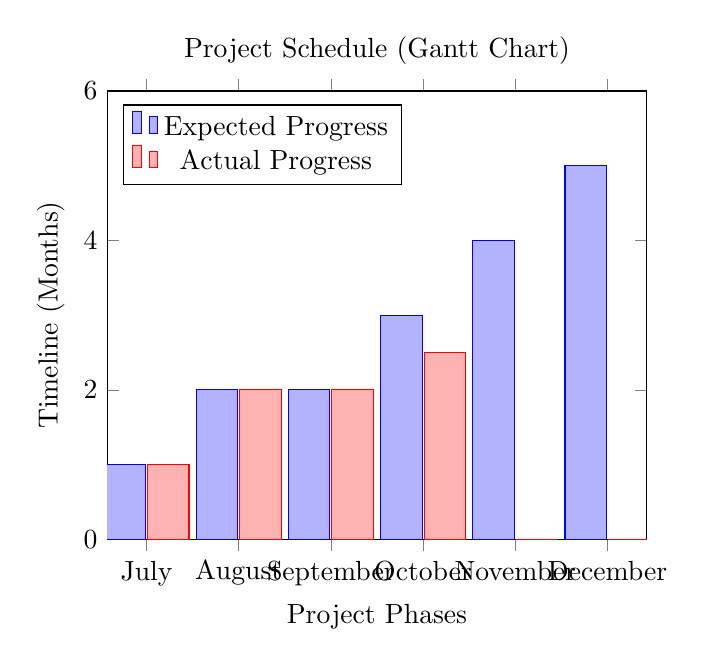
\begin{tikzpicture}
    \begin{axis}[
        title={Project Schedule (Gantt Chart)},
        xlabel={Project Phases},
        ylabel={Timeline (Months)},
        symbolic x coords={July, August, September, October, November, December},
        xtick=data,
        ybar=0.7,
        ymin=0, ymax=6,
        bar width=15pt,
        enlarge x limits={abs=0.5cm},
        legend pos=north west
    ]
    \addplot coordinates {(July, 1) (August, 2) (September, 2) (October, 3) (November, 4) (December, 5)};
    \addlegendentry{Expected Progress}
    
    \addplot coordinates {(July, 1) (August, 2) (September, 2) (October, 2.5) (November, 0) (December, 0)};
    \addlegendentry{Actual Progress}
    \end{axis}
\end{tikzpicture}
\end{center}

\section{Risks and Mitigation}
The project has encountered several risks that could affect its schedule and budget:
\begin{itemize}
    \item \textbf{Risk:} Delays in API integration.
    \item \textbf{Mitigation:} Additional resources have been assigned to focus on API development.
    \item \textbf{Risk:} Potential delays in acceptance testing due to late development completion.
    \item \textbf{Mitigation:} Testing schedules will be adjusted to run in parallel with the remaining development work.
\end{itemize}

\section{Next Steps}
The following tasks are priorities for the next project phase:
\begin{itemize}
    \item Complete API integration by October 1, 2024.
    \item Begin testing before November 1, 2024.
    \item Ensure system implementation by December 2024.
\end{itemize}

\section{Conclusion}
In conclusion, the ABC project is progressing despite some minor delays in development. We are confident that the project will meet the revised schedule, and API integration is expected to be completed soon. Additional resources have been allocated to ensure that the testing and implementation phases remain on track.

\end{document}
